\chapter{Uitbreidingen} \label{uitbreidingen}

Het eindresultaat van onze module is een afgerond geheel en is dus ook bruikbaar. Er zijn echter nog enkele mogelijke uitbreidingen die wij voor ogen zagen. Deze hebben wij niet ge\"{i}mplementeerd wegens tijdsgebrek. We sommen in dit hoofdstuk enkele van deze uitbreidingen op en bespreken hoe wij ze eventueel zouden implementeren.

\section{Keuze van interval bij automatisch ophalen}
Onze huidige module voorziet een alternatieve vorm van de CoAP-\textit{observe} voor CoAP-resources die niet \textit{observable} zijn. Een gebruiker kan namelijk waarden periodiek laten ophalen, dit gebeurt aan de hand van opeenvolgende \textit{GET requests} waartussen een bepaald interval ligt. In onze module bedraagt die een hardgecodeerd aantal seconden (namelijk 5). Men zou echter de module gebruiksvriendelijker en meer configureerbaar kunnen maken door de gebruiker het interval te laten kiezen. Dit zou gelijkaardig kunnen gebeuren aan de keuze van het polling interval, eerder besproken in paragraaf \ref{rest}.

\section{Opvragen devices in subnetwerk met resource directory} \label{resourceDirectory}
Eerder werd al uitgelegd hoe \textit{resource discovery} in zijn werk gaat (Zie paragraaf \ref{resourceDiscovery}). Men kan dit principe doortrekken op subnetwerkniveau. Wanneer op een subnetwerk een \textit{resource directory} voorzien is
kunnen \textit{embedded devices} er hun \textit{well-known/core}'s in plaatsen. De module zou dan de gebruiker een lijst kunnen presenteren die alle aanwezige \textit{devices} in het subnetwerk opsomt, samen met de aangesloten resources. Men zou ook hier weer modulair kunnen werken en de \textit{devices} voorstellen als instanties van het \textit{contenttype} CoAP \textit{device}.\\

Nog een ander mogelijk alternatief dat overwogen werd is het sturen van een \textit{broadcast} op het subnetwerk. Deze \textit{broadcast} bevat dan een \textit{GET request} die de \textit{well-known/core} opvraagt van elk \textit{embedded device} in het subnetwerk. Het nadeel bij deze benadering is dat een \textit{broadcast} zeer belastend is voor het subnetwerk. Bovendien is het niet de bedoeling dat als een gebruiker ge\"{i}nteresseerd is in een ander subnetwerk, dat die belasting zomaar kan worden uitgevoerd. Wanneer men echter gebruik maakt van een \textit{resource directory} kan men bovendien beslissen welke \textit{embedded devices} publiek worden gemaakt, wat de beveiliging en belasting van het subnetwerk ten goede komt.

\section{Conditional observe}

Het principe van een \textit{conditional observe} is een uitbreiding van de standaard CoAP \textit{observe}. Het werd mede ontwikkeld door iMinds en wordt omschreven in een aparte \textit{draft}, namelijk de CoAP \textit{Conditional Observe draft} (huidig versie 3) \cite{coapConditionalObserveDraft}.\\

Een \textit{conditional observe} werkt net als een gewone CoAP \textit{observe} met dat verschil dat een waarde pas naar de client wordt opgestuurd wanneer de waarde aan een bepaalde voorwaarde voldoet. Dit kan bijvoorbeeld een temperatuur zijn waarvan je pas op de hoogte wilt gesteld worden wanneer die hoger wordt dan twintig graden Celsius.
Voor de \textit{conditional observe} wordt optie nummer 18 gebruikt. Deze optie moet steeds vergezeld worden van een gewone \textit{observe} optie (nr. 6) aangezien deze er een extensie van is.

\begin{figure}[h!]
\centering
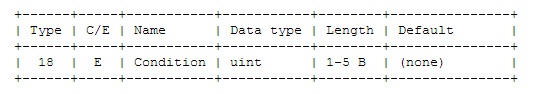
\includegraphics[width=0.8\textwidth]{fig/conditional}
\caption{Conditional observe optie (Option Delta 18)}
\end{figure}

De waarde kan vari\"{e}ren in lengte van \'{e}\'{e}n tot vijf bytes en bestaat uit de volgende onderdelen:
\begin{itemize}
\item TYPE: Beschrijft het type van de voorwaarde, bijvoorbeeld groter dan, kleiner dan, is gelijk aan,...
\item R: In een \textit{request} duidt deze bit aan of de client de notificaties als CON (1) of NON (0) verkiest. In een response duidt deze bit aan of de server bereid is om in te gaan op het verzoek van de \textit{client} om het betreffende soort berichten te sturen.
\item V: Deze twee bits duiden aan wat het type van de voorwaarde is (\textit{Integer}, tijdsduur in seconden of \textit{float}).
\item VAL: De waarde van de voorwaarde, de lengte hiervan kan vari\"{e}ren van \'{e}\'{e}n tot vier bytes.
\end{itemize}

\begin{figure}[h!]
\centering
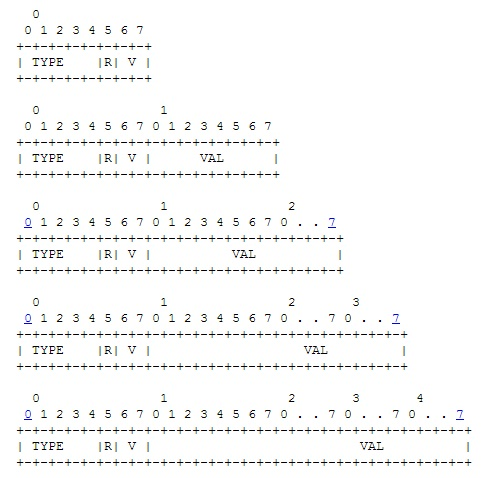
\includegraphics[width=0.8\textwidth]{fig/conditional_format}
\caption{Conditional observe optie formaat}
\end{figure}

\subsection{Keep-alive}

Men kan gebruik maken van de \textit{Keep-alive} optie om er zeker van te zijn dat de \textit{client} nog deel uitmaakt van de lijst van \textit{observers}. Het betreft hier optie 30.\\

\begin{figure}[h!]
\centering
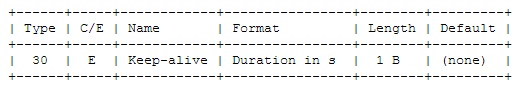
\includegraphics[width=0.8\textwidth]{fig/keep_alive}
\caption{De Keep-alive optie met Option Delta 30}
\end{figure}

Wanneer een \textit{client} een \textit{Keep-alive} optie meestuurt, vraagt die aan de server te bevestigen dat de \textit{client} nog tot de lijst met \textit{observers} behoort. En dit telkens wanneer een bepaald interval, meegegeven door de \textit{client} in de optie, verstrijkt en er in dat interval geen notificaties of enkel NON-berichten ontvangen zijn. De server stuurt dan een leeg bericht op, de voorwaarde werd immers niet voldaan.

\section{Custom Entity} \label{customEntity}
We gebruiken de \textit{Entity API} al voor manipulatie van content. Wat er nog mee mogelijk is, is het ontwerpen van een eigen \textit{entity}. Dit is toepasbaar op de waarden van resources. Momenteel worden waarden opgeslagen in de tabel coap\_resource\_values. Deze tabel wordt bij installatie aangemaakt en het manipuleren ervan wordt door onze eigen code afgehandeld. Als we een \textit{entity} coap\_resource\_value maken, worden de waarden nog steeds in dezelfde tabel opgeslaan maar kunnen we de manipulatie ervan laten gebeuren door de functies die de \textit{Entity API} aanbiedt. Een bijkomend voordeel is dat we \textit{custom views} kunnen maken van \textit{entities}. Gebruikers kunnen dan zelf \textit{custom views} van waarden aanmaken. Een gebruiker kan dus bijvoorbeeld alle waarden van 5 mei tot 5 juni opvragen.\\
Een nuttig voorbeeld van het aanmaken van een eigen \textit{entity} in code vind je in de module \textit{Model Entities} \cite{modelEntities}.\\

Een bijkomende uitbreiding is het gebruik van de module \textit{Entity Reference} \cite{entityReference}. Omdat we zelf een tabel cre\"{e}ren zonder aan Drupal te zeggen dat deze een speciale betekenis heeft, staan we zelf in voor de visualisatie van de waarden. Maar door een eigen \textit{entity} te maken kunnen we de waarden weergeven door gebruik te maken van een nieuw veld dat ge\"{i}ntroduceerd wordt door de \textit{Entity Reference}module.

\section{Interface Description}
Het attribuut if (\textit{interface description}) van het \textit{CoRE Link Format} kan info bevatten over welke methodes deze resource ondersteunt. Momenteel wordt deze info opgeslagen maar nog niet gebruikt. Deze informatie kan gebruikt worden om de methodes (GET, PUT, POST en DELETE) niet voor alle resources beschikbaar te laten zijn. De verschillende waarden en hun betekenis die het attribuut kan aannemen vind je in de \textit{CoRE Interfaces draft} \cite{coreInterfaces}.

\section{Configuratie op maat} \label{configuratie}
Bij installatie wordt een pagina voor configuratie voorzien. Deze kan je bereiken door eerst op '\textit{Configuration}' te klikken en dan op 'CoAP \textit{resource settings}'. Enige configuratieinstellingen komen hier te staan. Om de pagina die getoond wordt aan passen moet je de functie coap\_resource\_admin\_settings() in coap\_resource.module aanpassen.
\begin{figure}[h!]
\vspace{10pt}
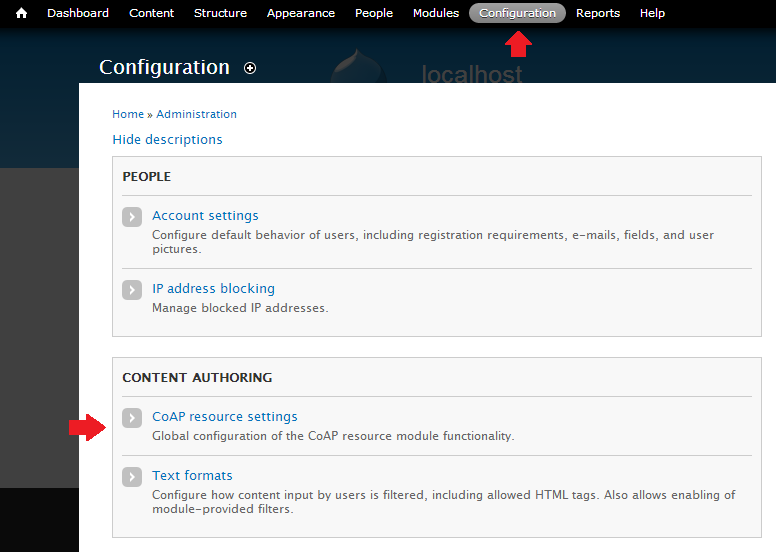
\includegraphics[width=1\textwidth]{fig/Configuratie}
\vspace{-30pt}
\caption{Navigatie naar de configuratiepagina als deze voorzien wordt}
\vspace{-10pt}
\end{figure}

\section{View Modes}
De content die we aanbieden wordt op elke pagina op dezelfde manier getoond. Door gebruik te maken van \textit{view modes} kunnen we hier verandering in brengen. Wanneer content van het type coap\_resource getoond wordt, kan je er verschillende functies op uitvoeren en zie je een \textit{history}tabel. Maar soms zou het handig zijn als je enkel de \textit{history}tabel ziet. Een complete \textit{tutorial} met uitleg vind je online \cite{viewMode}.

\section{DNS}
Het programma werkt enkel met IP-adressen. Door gebruik te maken van de PHP-functies \textit{gethostbyaddr(string \$ip\_addr)\cite{hostByAddr}} en \textit{gethostbyname(string \$hostname)}\cite{{hostByName}} kunnen \textit{hostnames} gebruikt worden i.p.v. hun respectievelijk IP-adres.

\section{Help}
Een standaard hulppagina kan voorzien worden door \textit{hook\_help} te implementeren. Deze kan opgevuld worden met de handleiding.
\begin{figure}[h!]
\vspace{10pt}
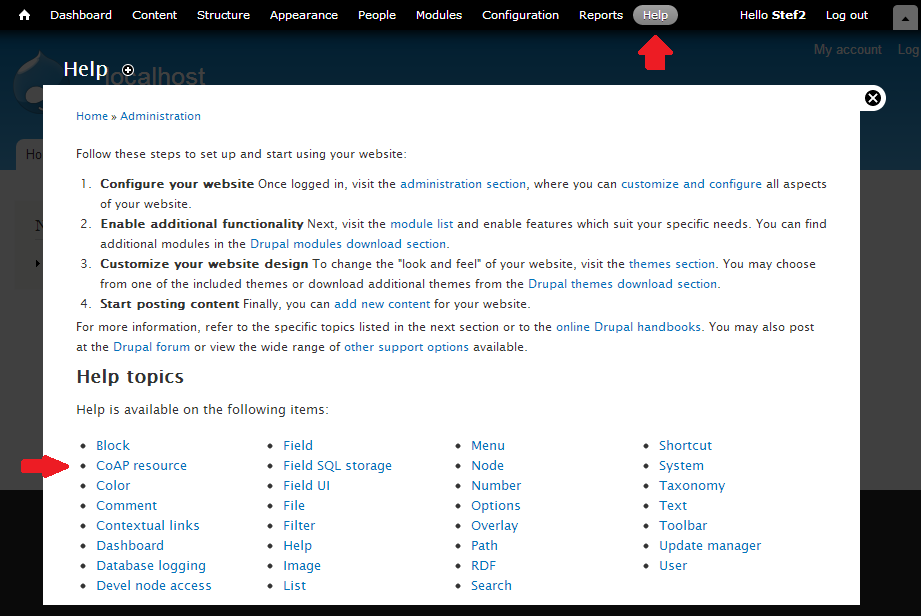
\includegraphics[width=1\textwidth]{fig/Help}
\vspace{-30pt}
\caption{Navigatie naar de hulppagina als deze voorzien wordt}
\vspace{-10pt}
\end{figure}

Er kan ook gebruik gemaakt worden van de \textit{Advanced Helpmodule} \cite{advancedHelp}. Wanneer deze module \textit{enabled} is, kan je hulppagina's opslaan in HTML-formaat en deze in je moduledirectory zetten. Deze module maakt ook het gebruik van pop-ups mogelijk en laat de administrator van de website beslissen voor wie de hulp beschikbaar moet zijn. We laten het aan de lezer over om alle mogelijkheden van deze module te bekijken.
\section{Block Options} \label{unsupportedBlockOptions}
Voor optie 28 (Size) en 27 (Block1) bieden we nog geen ondersteuning, momenteel worden ze genegeerd. Block1 hebben we reeds besproken in \ref{blocks}. De Size-optie wordt voor meerdere dingen gebruikt, maar ze hebben allemaal een verband met een schatting van de grootte van de resource representatie:
\begin{itemize}
\item In een request: om aan de server te vragen of hij een schatting meestuurt met zijn response. Hier moet als waarde 0 gebruikt worden.
\item In een response met een Block2-optie: om de schatting van de server aan te geven.
\item In een response met een Block1-optie: om de schatting van de client aan te geven.
\end{itemize}
De \textit{client} of server kan aan de hand van de schatting beslissen om grotere of kleinere \textit{blocks} door te sturen. Deze optie is niet verplicht te ondersteunen dus moet er rekening gehouden worden met dat de server of \textit{client} deze optie negeert.

\section{Anonieme gebruikers}
Momenteel worden anonieme gebruikers niet meer ondersteund. Er is wel een analyse uitgevoerd hoe ze best ge\"{i}mplementeerd worden. Voor anonieme gebruikers is het beter om zelf geen gegevens naar de databank te schrijven. Dit om ervoor te zorgen dat de databank niet overspoeld wordt met data.

Anonieme gebruikers hebben als \textit{user-ID} (uid)\nomenclature{uid}{user-ID} het getal 0. Anders dan gewone gebruikers die een uniek uid hebben kan je anonieme gebruikers hier niet op onderscheiden. Gebruikers hebben ook een \textit{session-ID} (sid)\nomenclature{sid}{session-ID} dat wel uniek is voor alle gebruikers. Nu moeten we de gegevens van de anonieme gebruiker bijhouden op een plaats die overal toegankelijk is maar dit mag niet de databank zijn. Daarom wordt er gebruik gemaakt van de sessievariabele \cite{sessionVariable} \$\_SESSION. Deze variabele is een PHP-tabel en het ligt voor de hand deze te indexeren op de sid. Alle gegevens worden nu best opgeslagen en aangesproken op volgende manier: \$\_SESSION[\$sid] met \$sid een variabele die de sid van de gebruiker bevat. 